\chapter{Implementation}\label{ch:sample-chapter}
\section{Development Environment}

\subsection{Tools and Technologies} \label{sec:tools-and-technologies}
We decided to implement the web proxy service with Intel SGX. The decision was influenced mainly by the previous knowledge of the technology by me and by the fact that Yoshimichi had already developed similar projects with Intel SGX. 

Intel-related technologies and corresponding versions:
\begin{itemize}
    \item \textbf{Intel SGX Version:} 2.4
    \item \textbf{Intel Attestation Service via EPID \cite{intelSGXattesationservice} API Version:} 5
\end{itemize}

The development and testing phases were carried out on a server provided by the System Security Group at ETH Zurich.

The server specifications are as follows:
\begin{itemize}
    \item \textbf{Operating System:} Ubuntu 20.04.6 LTS x86\_64
    \item \textbf{Kernel:} 5.4.0-97-generic
    \item \textbf{CPU:} Intel Pentium Silver J5005 (4 cores @ 1.500GHz)
    \item \textbf{Memory:} 5218 MiB
    \item \textbf{Enclave Page Cache (EPC) Size:} 128 MB
\end{itemize}

To ensure a stable and consistent environment for developing the web proxy service, the development and testing was carried in a Docker container running Ubuntu 18.04. This specific Ubuntu version was selected to ensure full compatibility with the Intel sgx-ra-tls library later described.

The development was done in C and the build is done via Makefiles. The choice of the programming language was highly influenced by the previous knowledge of the language compared to other choices such as Rust or C++ and, more significantly, by the amount of other Intel SGX Enclave projects that can be found online written using the same language. 

\subsection{Setting Up the Environment}
The environment setup process is documented in the codebase README.

Note that the remote attestation mechanism used in this project relies on Intel® SGX Attestation Service using Enhanced Privacy ID (EPID)\cite{johnson2016intel}. However, this service is scheduled for discontinuation: Development Access will be terminated on September 29, 2024, and Production Access on April 2, 2025, as detailed in this communication \cite{intelSGX-IAS-EOL}. 

Nevertheless, the library used in this project also supports Data Center Attestation Primitives (DCAP)\cite{dcap}, another attestation mechanism for Intel SGX, which will remain available and is not affected by this discontinuation.

\section{Custom Proxy Instead of Existing Solutions}
At the beginning of the project, using an open-source proxy or web server implementations was considered. However, it turned out that modifying these existing solutions to fit our specific design would be too complicated and time-consuming. So, it was decided that building a custom proxy from scratch would be easier and better suited to the project's needs.

\subsection{Proof of Concept Using Libraries}
Before engaging in the complex task of direct development with Intel SGX, we first assessed the feasibility of the approach using an integration layer: Gramine \cite{gramine}. This initial phase aimed to achieve two objectives: first, to determine if it was possible to fetch a website from within an enclave and serve it to users seamlessly, and second, to evaluate whether the enclave could support this operation with minimal overhead.

Gramine is described as a lightweight guest OS designed to run a single Linux application with minimal host requirements \cite{gramine}. By leveraging Gramine, it was possible to use the libraries \texttt{libhttpd} and \texttt{libcurl} within the enclave without any change to the library themselves. After resolving issues with the \texttt{manifest.template} file to mount necessary files for domain resolution and HTTPS requests, these libraries performed as expected. Thanks to these two libraries, it was possible to develop a basic web proxy service with just over 100 lines of code. This service uses HTTP to communicate to the clients and HTTPS to communicate to HTTPS-abled backend servers. 

\subsection{Challenges with Libraries Integration}
Intel SGX enclaves are isolated from the host operating system and do not have direct access to system calls. This isolation enhances security by preventing enclaves from performing privileged operations directly through the system call interface, thereby protecting against potential rogue OS interactions.

The above implementation leverages two libraries that do not work directly in an Intel SGX enclave due to their dependence on syscalls. In order to fix this issue and make the libraries working it is needed to define all the required system calls inside the enclave. The system calls can be provided with two strategies: by callings corresponding OCALLs or by implementing them direclty within the enclave, when possible.
Another factor to keep in mind is the complexity and size of these libraries, as well as the unclear internal logic of their functions. Modifying their underlying mechanisms to support a stream-based approach would be highly challenging.

Consequently, to maintain control over all the underlying logic and avoid excessive effort, it was decided to avoid the use of these two libraries in the final implementation.

\subsection{Using sgx-ra-tls library}
At this stage, developing a functional Intel SGX-based web proxy solution appeared to require manual implementation of several components: socket connections establishment, TLS handshakes with Remote Attestation (RA), HTTP protocol handling, and web proxy functionality. As a reader can probably tell, implementing these protocols from scratch, particularly TLS with RA, would be exceedingly difficult and time-consuming.

Therefore we decided to base the web proxy off of the \texttt{sgx-ra-tls} library \cite{sgx-ra-tls}. This library is an implementation of  an integration of Intel SGX Remote Attestation into the TLS connection setup. This library provides three implementations based on SSL libraries: wolfSSL, mbedtls, and OpenSSL.

The implementation based on wolfSSL was picked due to the fact that the library comes with an example of client and server applications written in C using the wolfSSL implementation. This implementation supports both IAS and DCAP Remote Attestation and constitutes a perfect base to develop an enclave supporting RA-TLS in Intel SGX. 

It is important to report that this library has been discontinued since December 20, 2022. Due to the lack of alternative open-source libraries integrating RA with TLS for Intel SGX and thanks to the fact that this library still works correctly, it was decided to go forward with it.
In order to avoid compatibility issues, it was made sure that the development environment versions used were the same that were lastly supported by the library. The versions are reported in Section \ref{sec:tools-and-technologies}.

\subsection{IAS instead of DCAP}
We decided to use IAS instead of DCAP, despite IAS being scheduled for deprecation as reported in \cite{intelSGX-IAS-EOL}. This decision was influenced by the simpler setup process for IAS, which can be completed in a few minutes compared to the more complex setup required for DCAP. The property of performing RA over TLS remains almost the same from a client perspective regardless of the choice between IAS and DCAP. Simplifying, the only difference is that with IAS there is one single root CA to be used to verify the report signature, while with DCAP, there is not a single root certificate, but different certificates could be used for different enclaves.

\section{Implementation Details}

\subsection{Enclave functionality via OCALLs or ECALLs}
The implementation of the service functionality inside the enclave can be approached in two ways (or a mixture of the two): either by performing all operations in the untrusted environment and only invoking the Enclave for sensitive operations via ECALLs, or by having the Enclave manage everything, using OCALLs only when system calls are necessary.

No matter the apporach, the number of ECALLs/OCALLs needs to be minimized for better performance. Therefore, the number of ECALLs and OCALLs would be the same regardless of the approach. It was decided to opt for the latter design (many OCALLs): this approach ensures that the Enclave maintains full control over the workflow, minimizing the exposure of ECALLs to the potentially malicious untrusted environment.

\subsection{Stream-based Data Forwarding and URL-rewriting}
The data forwarding mechanism is implemented as follows:

\begin{itemize}
    \item \textbf{From client to backend server:} The client's request is first fully received by the enclave before taking any action. This was not implemented in a stream-based fashion because the enclave needs to determine how to handle the request---whether to serve the welcome page or forward it to the backend server. In the latter case, the full URL must be constructed or retrieved before processing.
    
    \item \textbf{From backend server to client:} Responses are forwarded chunk by chunk as they are received, with URLs rewritten as needed. A chunk is defined as an arbitrary number of bytes, in the current implementation 4096 bytes, and correspond to the buffer used to receive data from the backend.
\end{itemize}

The URL rewriting is implemented similarly to what is described in the design section. The only difference is that the \texttt{modified\_original\_domain} of the rewritten URL is not modified, e.g., \texttt{sub.example.com} does not get modified and it will be used as it is, with the dots. 

Developing the URL rewriting algorithm was particularly challenging. Given the potential impact of URL rewriting on the web proxy service's performance, the algorithm was designed keeping efficiency in mind.

\subsubsection{Handling Split Tags Across Chunks}
One of the main challenges in developing this algorithm was ensuring it could handle cases where a tag begins in one chunk and ends in the next, or where the start of a tag itself is split across two chunks. To address this, the URL rewriting function takes both the current chunk and the next chunk in the stream as input. In situations like these, the next chunk is used to complete the URL rewriting. Although the algorithm does not rewrite URLs that span more than two chunks, this should not be common, given a chunk size of, for instance, 4096 bytes.

\subsubsection{Efficient Chunk Scanning for Performance}
Another challenge was designing the algorithm to be efficient. The core functionality involves scanning each chunk to be rewritten. For every opening tag (e.g., \texttt{href="}), the algorithm locates the corresponding closing tag (e.g., \texttt{"}) and rewrites the content between them according to the URL rewriting rules outlined in the previous chapter. The efficiency of this process was carefully considered, for instance by avoiding scanning the chunk multiple times.

\subsection{UX}
I kept the user experience (UX) of the implemented web proxy intentionally minimal. Upon connecting to the web proxy, the user is presented with a simple interface featuring a form where they can submit the URL they wish to visit, as shown in Figure \ref{fig:homepage}.

The web proxy navigation is designed to be as transparent to the user as possible as shown in \ref{fig:website-navigation}. This is possible thanks to the fact that the enclave does not inject any custom HTML into the visited pages. The only indication that the user is navigating through the web proxy is in the browser's address bar, where the connection to the web proxy is visible.

\begin{figure}[h!]
    \centering
    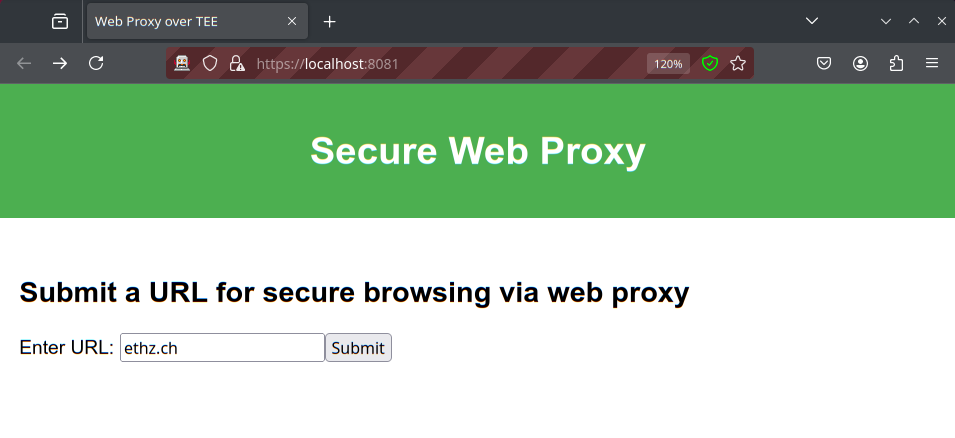
\includegraphics[width=1\linewidth]{media/homepage.png}
    \caption{Homepage of the web proxy.}
    \label{fig:homepage}
\end{figure}

\begin{figure}[h!]
    \centering
    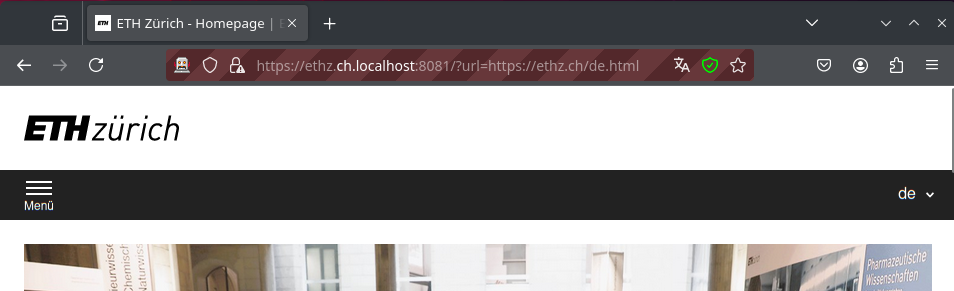
\includegraphics[width=1\linewidth]{media/website-navigation.png}
    \caption{ETH website visited through the web proxy.}
    \label{fig:website-navigation}
\end{figure}

\subsection{Certificates Verification and Datetime inside the Enclave}
Root certificate pinning is implemented in the enclave to store the Root Certificate Authorities (CAs) needed to verify backend certificates. This is the fastest way to provide an enclave with the necessary Root CAs. An alternative method would be to set up a more complex mechanism to fetch Root CAs from a trusted source, which would allow the storage of only one certificate (to verify this source). However, this approach could create a single point of failure.

During the development phase, a significant amount of time was spent troubleshooting the persistent failures of TLS handshakes between the enclave and external servers. The root cause was eventually identified in the enclave not having the correct date, which led to certificates being deemed ``too new'' and therefore invalid. Securely obtaining the current time within an Intel SGX enclave is challenging due to its limited access to external resources, including system clocks. The primary difficulty lies in ensuring that the time source is trustworthy and immune to tampering, especially since enclaves operate in an untrusted environment.

Addressing this issue is complex and falls outside the scope of this project. As a temporary workaround, the date is currently hardcoded into the enclave's code.

\subsection{Enclave Certificate}
During the initialization phase, the enclave undergoes the Remote Attestation process via the Intel Attestation Service (IAS) and generates a self-signed certificate. This certificate includes the IAS report and its signature, which are used to verify the enclave's identity (MRENCLAVE). The IAS report binds the enclave's public key to its identity, and this binding can be validated using the Intel Root CA and the report signature. The public key is then used to self-sign the certificate, which will be used for all TLS connections between any client and the enclave.

\section{Browser Extension}

As previously discussed, the enclave uses a self-signed certificate. Consequently, when a user connects to the web proxy service via a browser, a warning is displayed indicating that the website is using a self-signed certificate. While it is theoretically possible for a user to manually verify the entire certificate chain and thus confirm the enclave's identity, this process requires significant time and expertise.

To address this issue, it was decided to developed a browser extension that automates the verification of the certificate chain used in the TLS connection between the browser and the enclave. The extension also clearly displays the enclave's identity (\texttt{MRENCLAVE}). However, is up to the user to check that the enclave's identity matches the expected value.

The simplified steps performed by the extension are as follows:
\begin{enumerate}
    \item Verify the signature of the report included in the TLS certificate using the Intel Root CA.
    \item Extract the public key from the report and compare it with the one used in the self-signed certificate.
    \item Extract and display the enclave's identity.
\end{enumerate}

The extension was developed for Firefox due to the browser's comprehensive developer tools, though it can be easily ported to other browsers. The source code is available in the project's codebase.

Figure \ref{fig:verified} shows the extension when verification is successful. In contrast, Figure \ref{fig:not-verified} shows the extension in the case of unsuccessful verification.

\begin{figure}[h!]
    \centering
    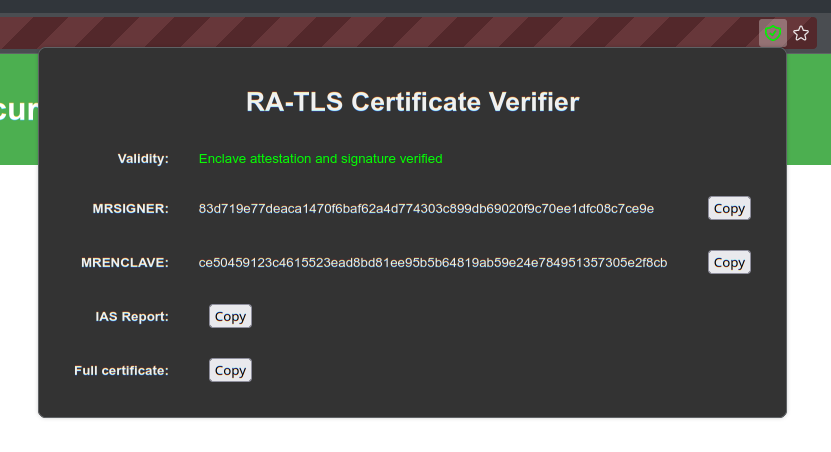
\includegraphics[width=1\linewidth]{media/verified.png}
    \caption{Successful verification of a certificate.}
    \label{fig:verified}
\end{figure}

\begin{figure}[h!]
    \centering
    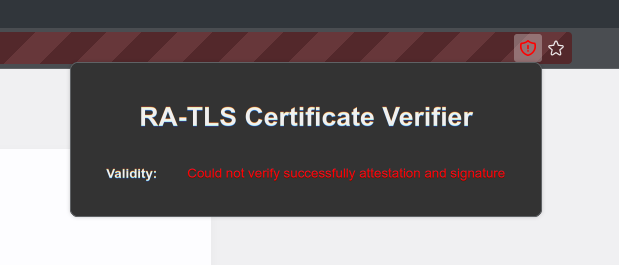
\includegraphics[width=1\linewidth]{media/not-verified.png}
    \caption{Unsuccessful verification of a certificate.}
    \label{fig:not-verified}
\end{figure}

\clearpage
\section{Differences With Design} \label{sec:differences-with-design}
Beyond the minor differences with the design previously outlined in this section, there are additional key differences worth noting:
\begin{itemize}
    \item DNS queries are not performed using DoT\cite{rfc7858}, DoH\cite{rfc8484}, or PDoT\cite{Nakatsuka_2019}, as these are beyond the scope of the project and would add unnecessary complexity to the implementation.
    \item Only GET requests are supported, and client request headers are not utilized when making requests to the backend.
    \item SNI encryption is not supported on the client side and is not employed when making requests to the backend servers.
\end{itemize}
